\documentclass[tikz,border=2pt]{standalone}
\usepackage{amsmath,amssymb}
\usepackage{pgfplots}
\pgfplotsset{compat=1.18}
\usetikzlibrary{arrows.meta}

\begin{document}
% f(x1,x2)=x1^2+x2^2, x0=(1,0), v=(3/5,4/5).
% h(t)=f(x0+t v)=1+6t/5+t^2; h'_+(0)=6/5. No gradient is needed.
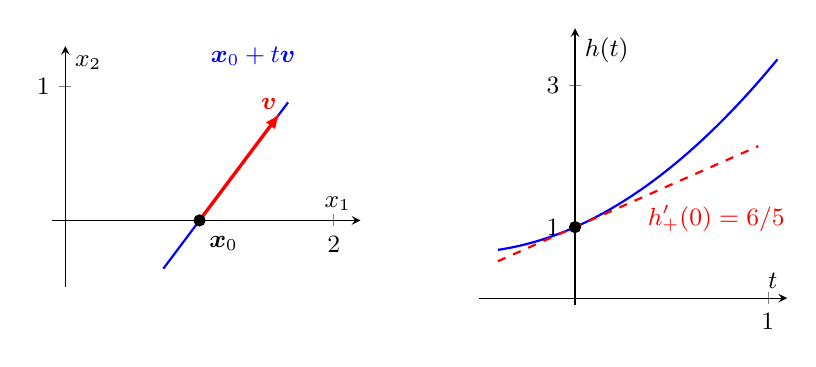
\begin{tikzpicture}[font=\small, >={Latex[length=2mm]}]
\begin{axis}[
  name=input, width=5.5cm, height=5.1cm,
  axis lines=middle, axis equal image,
  xmin=-0.1, xmax=2.2, ymin=-0.5, ymax=1.3,
  xtick={2}, ytick={1}, xlabel={$x_1$}, ylabel={$x_2$},
  clip=false
]
  \addplot[blue, thick, domain=-0.45:1.1] ({1+0.6*x},{0.8*x});
  \addplot[only marks, mark=*, black] coordinates {(1,0)};
  \node[below right] at (axis cs:1,-0.05) {$\boldsymbol{x}_0$};
  \draw[->, red, very thick] (axis cs:1,0) -- (axis cs:1.6,0.8);
  \node[red, above left, fill=white, inner sep=1pt] at (axis cs:1.6,0.8) {$\boldsymbol{v}$};
  \node[blue, above, fill=white, inner sep=1pt] at (axis cs:1.4,1.13) {$\boldsymbol{x}_0+t\boldsymbol{v}$};
\end{axis}
\begin{axis}[
  at={(input.east)}, anchor=west, xshift=1.5cm,
  width=5.5cm, height=5.1cm, axis lines=middle,
  xmin=-0.5, xmax=1.1, ymin=-0.1, ymax=3.8,
  xtick={0,1}, ytick={1,3}, xlabel={$t$}, ylabel={$h(t)$},
  clip=false
]
  \addplot[blue, thick, domain=-0.4:1.05, samples=80] {1+1.2*x+x^2};
  \addplot[red, dashed, thick, domain=-0.4:0.95] {1+1.2*x};
  \addplot[only marks, mark=*, black] coordinates {(0,1)};
  \node[red, below right, fill=white, inner sep=1pt] at (axis cs:0.36,1.35) {$h'_+(0)=6/5$};
\end{axis}
\end{tikzpicture}
\end{document}
